

% \titleformat{\subsection}
%   {\normalfont\Large\bfseries}{}{0em}{}

\section*{Part \uppercase\expandafter{\romannumeral1} Introduction to the Group Project}
\addcontentsline{toc}{section}{Part \uppercase\expandafter{\romannumeral1} Introduction to the Group Project} 
\setcounter{section}{1}

% ----- 1.1 Background and Objective

\subsection{Background and Objective}
In recent years, the concept of the "metaverse" has captivated the global imagination, 
presenting a fusion of the physical and virtual realms that expands the horizons of human creativity and innovation. 
The word \textit{"METAVERSR"} consists of two words, \textit{meta} and \textit{verse} (\textit{meta} comes from Greek, the prefix meaning transcendence and \textit{verse} meaning universe). 
It is a parallel world closely connected with the real world, a product of the development and integration of various technologies, 
the next stage in the development of the Internet, and a virtual living space with social attributes\cite{Survey_on_the_Metaverse}. 
As the digital and physical worlds intertwine, the metaverse has ignited a transformation across industries, propelling forward the digital economy.

However, despite this unprecedented growth and the dynamic nature of university environments—where innovation and the bridge between academia and industry thrive—there is an evident gap in the development of metaverse platforms tailored to the campus community. 
Existing designs often replicate the physical world without leveraging the unique potential of immersive and interactive metaverse experiences.

At the heart of this expansive vision lies a focal point of ingenuity ———— the 
\textit{AI Agent Driven Storytelling Game in Metaverse}. 
Our project meticulously crafted within the larger canvas of the metaverse campus community 
is the essence of our commitment to redefining the boundaries of technological integration, 
immersive experiences, and creative expression within the metaverse, 
which also represents the apex of our vision, embodying the convergence of high-quality creative content, 
artificial intelligence, and interpersonal interaction within the metaverse.

The objective of this project is to create a metaverse storytelling game that is tailored to the campus community,
which seamlessly intertwining technological prowess, immersive experiences, creative content integration, 
and its role as a nexus for educational and entrepreneurial exploration. Specifically the following:
\begin{itemize}
    \item [1)] 
    \textbf{immersive Metaverse platform:} The objective is to immerse users in a metaverse experience that goes beyond replication, enhancing reality. By strategically employing spatial computing and interactive elements, users actively participate in a narrative that unfolds within the metaverse campus. 
    This immersive quality blurs the lines between physical and virtual, delivering a transformative experience that transcends traditional virtual platforms.
    \item [2)]
    \textbf{Technology Innovation Fusion:} Artificial Intelligence agent-driven narrative games are developed using advanced AI and human interaction technologies 
    that go beyond traditional game concepts. Players can interact with state-of-the-art AI and experience narratives that dynamically adapt to their behaviors, 
    thus making metaverse and computer technology an integral part of their immersive metaverse experience.
    \item [3)]
    \textbf{Unleashing Creativity and Imagination:} As a beacon for creativity and imagination within the metaverse campus community, the AI Agent driven storytelling game offers a dynamic narrative that adapts to user input. Leveraging AI, the game becomes a virtual canvas for limitless expression and ideation, 
    encouraging faculty and students to explore uncharted realms of innovation and contribute to the unique culture of the metaverse campus.
    \item [4)]
    \textbf{Broader Metaverse Ecosystem:} With a dual emphasis on both entrepreneurial and scientific research attributes, the AI Agent driven storytelling game becomes a catalyst for cultivating digital economy growth. By fostering an environment where creativity meets technology, 
    the project contributes to entrepreneurial endeavors and the development of application services, potentially driving explosive growth in the digital economy. 
    This emphasis on both aspects ensures a comprehensive and impactful contribution to the broader metaverse ecosystem.
\end{itemize}

% ----- 1.2 Significance

\subsection{Significance}
In the modern landscape of technological advancement, the inception of "A Metaverse Campus Community - AI Agent Driven Storytelling Game in Metaverse" stands as a crucial and forward-thinking effort, 
underscored by its multifaceted significance within the real-world context. 
The growing metaverse phenomenon, characterized by the merging of physical and virtual realms, holds transformative potential across various sectors, requiring the development of tailored metaverse platforms. 
This project, situated at the intersection of academia and the metaverse, not only addresses a critical gap in existing metaverse designs but also represents a pioneering foray into uncharted territory.

The importance of this group project becomes evident when considering the current trajectory of the global metaverse and Generative AI industry. 
Projections indicate the market size of the metaverse to rise from \$ 209.77 billion in 2021 to a staggering \$ 716.5 billion by 2027\cite{Metaverse_Market_Size}. 
With the advent of ChatGPT, Generative AI is the most recent buzzword in the technological space, and the metaverse is a veteran within the advanced technology landscape. 
The Generative AI market size is expected to reach \$ 109.37 billion (CAGR 35.6\%) by 2030. The metaverse market is expected to surpass \$ 1.3 trillion (CAGR 45\%) by the same period. 
Despite setbacks from industry leaders like Meta (formerly Facebook) and Disney, the Metaverse still generates intrigue and funding interest, and the initiative assumes a role of paramount importance in steering the course of the digital revolution\cite{Saivasan2023-am}. 

Educational institutions, traditionally crucibles of innovation and intellectual exploration, have yet to fully embrace the immersive and interactive potential of the metaverse. 
This project bridges that gap by offering a metaverse experience customized for the campus community. 
By strategically employing spatial computing, interactive elements, and artificial intelligence, it aims to transcend the limitations of conventional virtual platforms. 
The immersive metaverse platform crafted within this initiative becomes not merely a replication of the physical world but a transformative space where reality is augmented, 
fostering an environment conducive to cutting-edge research, interdisciplinary collaboration, and experiential learning.

Beyond academia, the project's significance extends to broader societal and economic realms. 
As the metaverse becomes an integral part of the digital economy, this initiative positions itself as a catalyst for cultivating digital entrepreneurship and scientific research. 
The artificial intelligence-driven narrative games developed herein represent a fusion of advanced AI technologies and human interaction, propelling the metaverse beyond traditional gaming concepts. 
This innovation has the potential to redefine user engagement and narrative experiences, setting new standards for immersive storytelling in digital environments.

Crucially, the project's emphasis on creativity and imagination within the metaverse campus community underscores its role as a harbinger of innovation. 
By providing a dynamic narrative canvas that adapts to user input through AI, it becomes a conduit for limitless expression and ideation. 
Players are empowered to explore uncharted realms of innovation, contributing to the unique cultural fabric of the metaverse campus. 
This, in turn, ensures that the project not only meets the immediate needs of the academic environment but also has a lasting impact on the evolving nature of creativity and expression in the metaverse.

In conclusion, "A Metaverse Campus Community - AI Agent Driven Storytelling Game in Metaverse" emerges as an essential undertaking in the real-world context, 
poised to redefine the boundaries of technological integration, immersive experiences, and creative expression. 
Its comprehensive approach, from immersive metaverse platforms to technology innovation fusion and its broader contributions to the metaverse ecosystem, positions it as a transformative force at the forefront of the digital revolution. 
As the global metaverse industry continues its exponential growth, this project stands as a beacon, illuminating the path toward a future where academia and the metaverse converge to shape the next frontier of innovation and human experience.


% ----- 1.3 Project Composition

\subsection{Project Composition}
\begin{itemize}
    \item \textbf{Xiaoyun ZHONG - Multi-AI Agent and Multi-Player Perceptual Interaction System and Decision-Making in Metaverse Narrative Game:}
    The research project addresses the intricate dynamics of multi-AI agents and the complexities introduced by multi-player perceptual interactions within the realm of a Metaverse narrative game, 
    wherein decision-making emerges as a distinctive form of interaction crucial to advancing the narrative. With a specific focus on perceptual interactions, 
    the work aims to enrich the metaverse experience by exploring the nuanced dynamics between multi-AI agents and human participants, where decision-making serves as a pivotal mechanism propelling the narrative forward, 
    aiming to enhance the immersive quality of the metaverse experience through advanced perceptual interactions and strategic decision-making.
    \item \textbf{Peixian Ma - Multi-Agent Capability Optimization Based on Causal Reasoning in AI Agent Narrative Game System:}
    The research project revolves around the optimization of multi-agent capabilities through the application of causal reasoning within the AI agent narrative game system. 
    By leveraging causal reasoning, this project aims to enhance the efficiency and effectiveness of multi-agent interactions, 
    thereby elevating the overall gameplay experience and contributing to the seamless integration of AI-driven narratives within the metaverse.
    \item \textbf{Yuelu LI - Exploring the Methods and Impact of Interactive Storytelling with AI Agent Intervention in the Metaverse:}
    The research project delves into the methods and impact of interactive storytelling within the metaverse, 
    accentuating the integration of AI agents. This research investigates the intricate balance between human agency and AI intervention. 
    It seeks to unravel the implications of AI-driven narrative elements on user engagement and the overall storytelling experience, 
    emphasizing the integral role of AI in shaping interactive narratives within the metaverse.
    \item \textbf{Zhihan GUO - Memory Generation and Decision Making of AI Agent in Storytelling Games:}
    The research project explores the fusion of multimodality and large language modeling within the context of memory generation and decision-making by AI agents in storytelling games. 
    This research incorporates the use of images as a means to store, acquire, and present information, adding a visual dimension to the cognitive processes of AI agents, 
    which also endeavors to decipher how AI agents create, store, and utilize memories to inform their decision-making processes and contributes to the broader understanding of how multimodal approaches enhance the adaptive nature of narrative experiences in storytelling games within the metaverse.
\end{itemize}

Collectively, these individual projects form a cohesive and comprehensive research initiative, addressing diverse facets of AI-driven storytelling, perceptual interactions, memory generation, decision-making, and multi-agent capabilities within the metaverse narrative game. 
This multidimensional approach ensures a holistic exploration of the metaverse's potential, emphasizing the integration of advanced technologies to redefine the boundaries of immersive experiences and creative expression.

% ----- 1.4 Project Connections

\subsection{Project Connections}
\begin{figure}
    \centering
    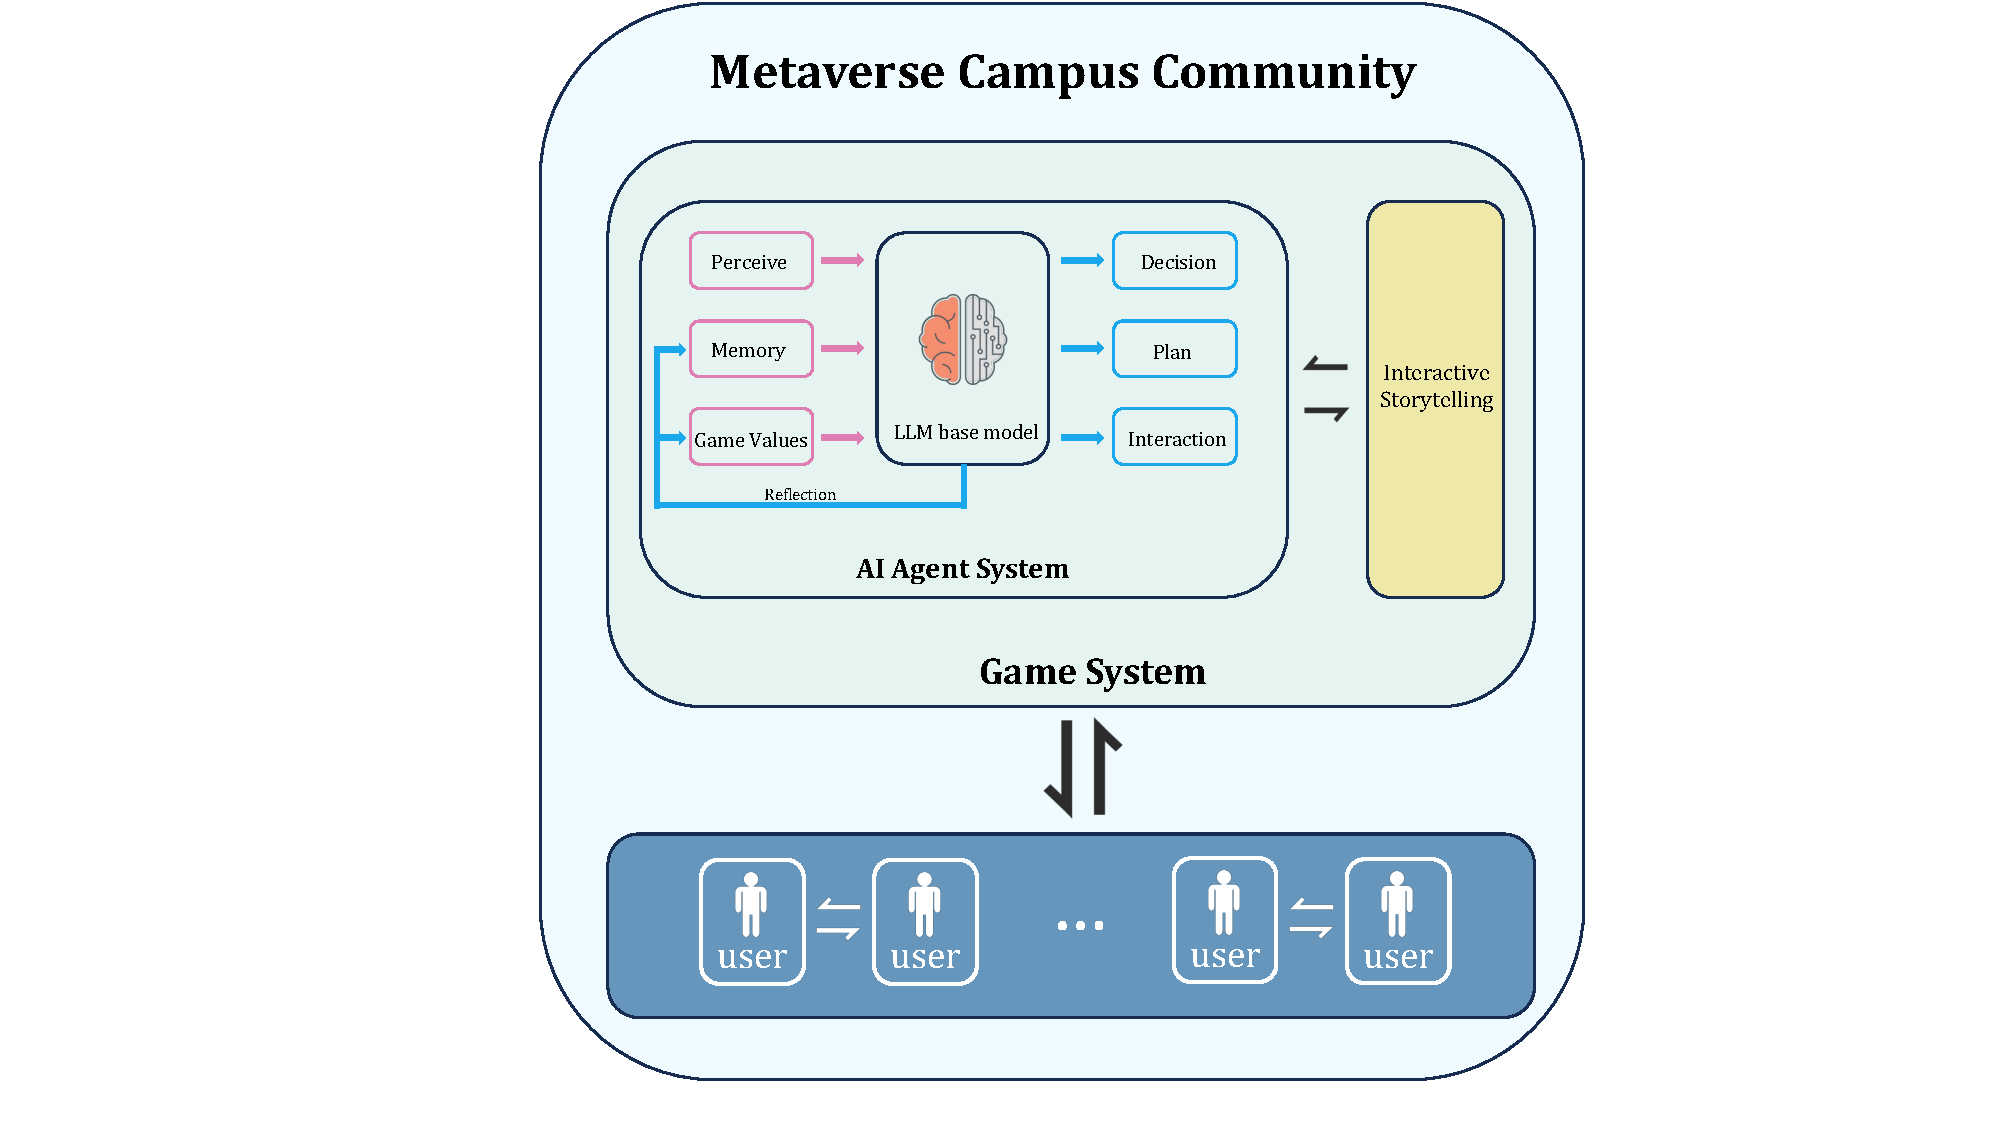
\includegraphics[width=0.8\textwidth]{image/Group-pipeline.pdf}
    \caption{Group Project Pipeline}
  \label{fig:Group_pipeline}
\end{figure}
To better articulate the components and linkages of the overall team project, 
Figure\ref{fig:Group_pipeline} illustrates the general pipeline of the entire project.
Our team project is primarily focused on the metaverse campus community environment, as an important creative content component, 
leveraging the creativity of generative AI and advanced human interaction technology to enhance the immersive experience. 
This aims to provide a more creative and personalized experience for the entire metaverse campus community. 
The user is the player within the game system, interacting with other players and the entire game system. 
The game system is mainly comprised of two parts, with the AI agent system centered on the LLM base model serving as the core functional area. 
It involves utilizing the basic operation process of the AI agent, including information collection, processing, and feedback functions. 
This includes inputting the agent's perceive, memory, and other game values from the outside, and after processing by the large language base model, 
generating outputs such as decisions, plans, and various interactions. 
Additionally, it updates the memory and game values within the system after reflection.

After introducing the pipeline and functional partitions of the entire team project, the connection and correlation between individual projects within the team and the team project becomes clearer. 
Roughly, individual projects can be categorized into the following four sections:
\begin{itemize}
    \item \textbf{Perception、Interaction and Decision-making of Multiple Generative Agents System(Xiaoyun ZHONG):}
    Xiaoyun ZHONG's project primarily addressing the AI agent system's perception, input game values, plan creation, and interactive aspects. 
    By focusing on the perception of the agent in the external environment and utilizing information to generate decisions, 
    ZHONG's work contributes significantly to the metaverse narrative game's overarching goal where AI agents dynamically engage with users, fostering an interactive and engaging storytelling experience. 
    The emphasis on interaction and decision-making serves as a critical link to driving the narrative forward, providing essential insights for the group project's development of an immersive and responsive AI-driven storytelling experience.
    \item \textbf{Causal Reasoning and Multi-Agent Optimization for Large Language Model interface(Peixian Ma):}
    Peixian Ma's project focuses on providing an interface to the Large Language Model (LLM) base model optimized using causal inference for the entire AI agent system. 
    Ma's work plays a pivotal role in ensuring that the necessary information processing modules within the AI agent operation are optimized through causal reasoning. 
    This optimization contributes to the efficiency and responsiveness of the entire metaverse narrative game system. 
    Ma's project thus establishes a critical connection within the group project by enhancing the underlying technology infrastructure and supporting the seamless operation of the AI agents, ultimately enriching the user experience within the metaverse.
    \item \textbf{Interactive Storytelling with AI Agents Intervention (Yuelu LI):}
    Yuelu LI's contribution to the group project is multifaceted, offering expertise in interactive tent creation and innovative strategies for integrating interactive storytelling with AI agents. 
    LI's project not only provides valuable insights into the design and implementation of an engaging AI agent interaction system within the metaverse but also extends the group project's scope by creating original metaverse interactive storytelling content. 
    By using the campus as a theme and case study, LI's work serves as an empirical example, enriching the group project's practical applications and further elevating the metaverse experience through thoughtful and engaging storytelling.
    \item \textbf{Multimodal Memory Generation and Decision-Making (Zhihan GUO):}
    Zhihan GUO's focus on multimodal memory generation and decision-making provides a vital connection to the broader vision of the group project. 
    GUO's research, which incorporates multimodality and large language modeling, enriches the metaverse narrative game by introducing a visual dimension to memory processes and decision-making by AI agents. 
    The utilization of images to store, acquire, and present information enhances the depth and adaptability of the narrative, aligning with the group project's commitment to pushing the boundaries of technological integration and creative expression within the metaverse.
\end{itemize}
The connection of the individual projects lies in their collective contribution to the overall metaverse narrative game system. 
The optimized model interface provided by MA is the processing core of the whole system, providing information processing functions for the functional modules of the other three, 
while at the same time the projects of the others need to be adjusted and optimized according to the characteristics of the model provided by MA; 
the system implemented by ZHONG design is closely connected with the memory module designed by GUO, and the decision-making function of the ai agent also needs to refer to the GUO memory module, 
and also needs to serve the narrative elements designed by LI, including narrative scenes, characters, plots and dynamic changes, etc. 
The decision-making function of the ai agent should also refer to the additional information provided by GUO's memory module and multimodality, and also need to serve the narrative elements designed by LI; 
GUO needs to refer to the interaction and perception module designed by ZHONG when designing the memory module and multimodality, and utilize the information to generate and store the corresponding memories, 
which also need to be in line with LI's narrative elements; LI needs to integrate the narrative elements and method into the AI Agent system design to fully utilize the Agent's narrative potential, ensuring a cohesive and responsive dynamic metaverse narrative experience. 
These individual projects come together to create a metaverse campus community that utilizes AI-driven storytelling to facilitate user engagement and push the boundaries of immersive experience and creative expression in the metaverse.


% ----- 1.5 Project Milestones
\subsection{Project Milestones}
List the key milestones at different stages of the group project implementation.

\begin{itemize}
    \item [1)] 
    \textbf{May 31, 2024 - Development and initial testing of individual functional modules:} 
    The initial milestone marks the first phase of the group's project implementation phase. Each group member will start developing their own functional modules before this time point to lay a solid foundation for a comprehensive Metaverse narrative game. 
    The focus will be on making and testing the basic functionality of the respective projects, ensuring that the AI agent driven storytelling game achieves its basic functionality. 
    When reaching this milestone, the basic functions of several main components of the entire team project should be initially implemented and presented, which is an important foundation.
    \item [2)]
    \textbf{September 30, 2024 - First generation prototype - integration of basic functional modules:} 
    As each functional module takes shape, the team project will begin to enter the integration phase. 
    This milestone involves the merging of various functions, including basic large-scale language model training results and interface access, the exploration and integration of AI agent system functions, and the attempt at interactive narrative mode, 
    and finally the creation of a metaverse narrative game demonstration prototype, including basic Preliminary integration results of functional modules. 
    The main goal is to demonstrate the fundamental characteristics of a metaverse narrative game, highlighting the synergies between different AI agent systems and their collective impact on the overall user experience, while revealing preliminary narrative elements and potential.
    \item [3)]
    \textbf{March 31, 2025 - Second Generation Prototype - Optimized Integration and Narrative Development:} 
    Building on the first generation prototype, the second milestone focuses on optimization and more comprehensive integration. 
    Team members will delve into improving prototypes, solving integration challenges, and enhancing the overall gaming experience. 
    This phase involves resolving issues that may arise during the integration process of the first-generation prototype, ensuring seamless collaboration between the AI agent system and the interactive narrative. 
    In addition, we will also work hard to gradually improve game functions and narrative design, deeply integrate narrative elements and interactive functions, and develop interactive narrative experiences that multiple players can participate in. 
    This milestone aims to achieve more detailed and immersive virtual world experiences by iteratively improving the initial prototype.
    \item [4)]
    \textbf{August 31, 2025 - Third Generation Prototype - Further Development, User Testing, and Iterative Optimization:} 
    The final milestone marks the refinement and progress of the Metaverse narrative game towards its third prototype. 
    At this stage, the focus turns to user testing to gather valuable feedback and insights. Team members will interact with users to learn about their experiences, preferences and suggestions. 
    This feedback loop will inform further development, leading to iterative optimizations designed to enhance user engagement, narrative depth, and overall gameplay. 
    This milestone highlights an iterative approach to ensuring Metaverse narrative games evolve into refined and user-centered experiences.
\end{itemize}

\begin{table}
  
    \begin{center}
  \def~{\hphantom{0}}
    \begin{tabular}{lccc}
        \hline
        \textbf{Time}  & \textbf{milestones} \\[3pt]
        \hline
         31/05/2024   & Development and initial testing of individual functional modules\\
         30/09/2024   & First generation prototype - integration of basic functional modules\\
         31/03/2025   & Second Generation Prototype - Optimized Integration and Narrative Development\\
         31/08/2025   & Third Generation Prototype - Further Development, User Testing, and Iterative Optimization\\
         \hline
    \end{tabular}
    \caption{Project Milestones}
    \label{tab:milestones}
    \end{center}
\end{table}

These carefully planned milestones provide a roadmap for the phased implementation of the group's projects, ensuring a systematic progression from individual module development to collaborative integration, optimization and user-driven refinement. 
Each stage contributes to the collective goal of creating an innovative and immersive virtual campus community where AI agent driven storytelling redefines the boundaries of interactive storytelling and technology integration.